\documentclass[00_doc.tex]{subfiles}
\begin{document}
    \subsection{Building Process}
    \begin{flushleft}
        To build the prototype, we modeled the base for the lamp (see Figure ~\ref{fig:blossomBaseModel}). Therefore, we used
        Autodesk. After doing so, we used a milling machine. We only had to convert the 3D model into a ".iges"-file.
        The result of the milling process can be seen in Figure ~\ref{fig:blossomBase}.
    \end{flushleft}

    \begin{figure}[H]
        \centering
        \begin{subfigure}{.45\textwidth}
        \centering
        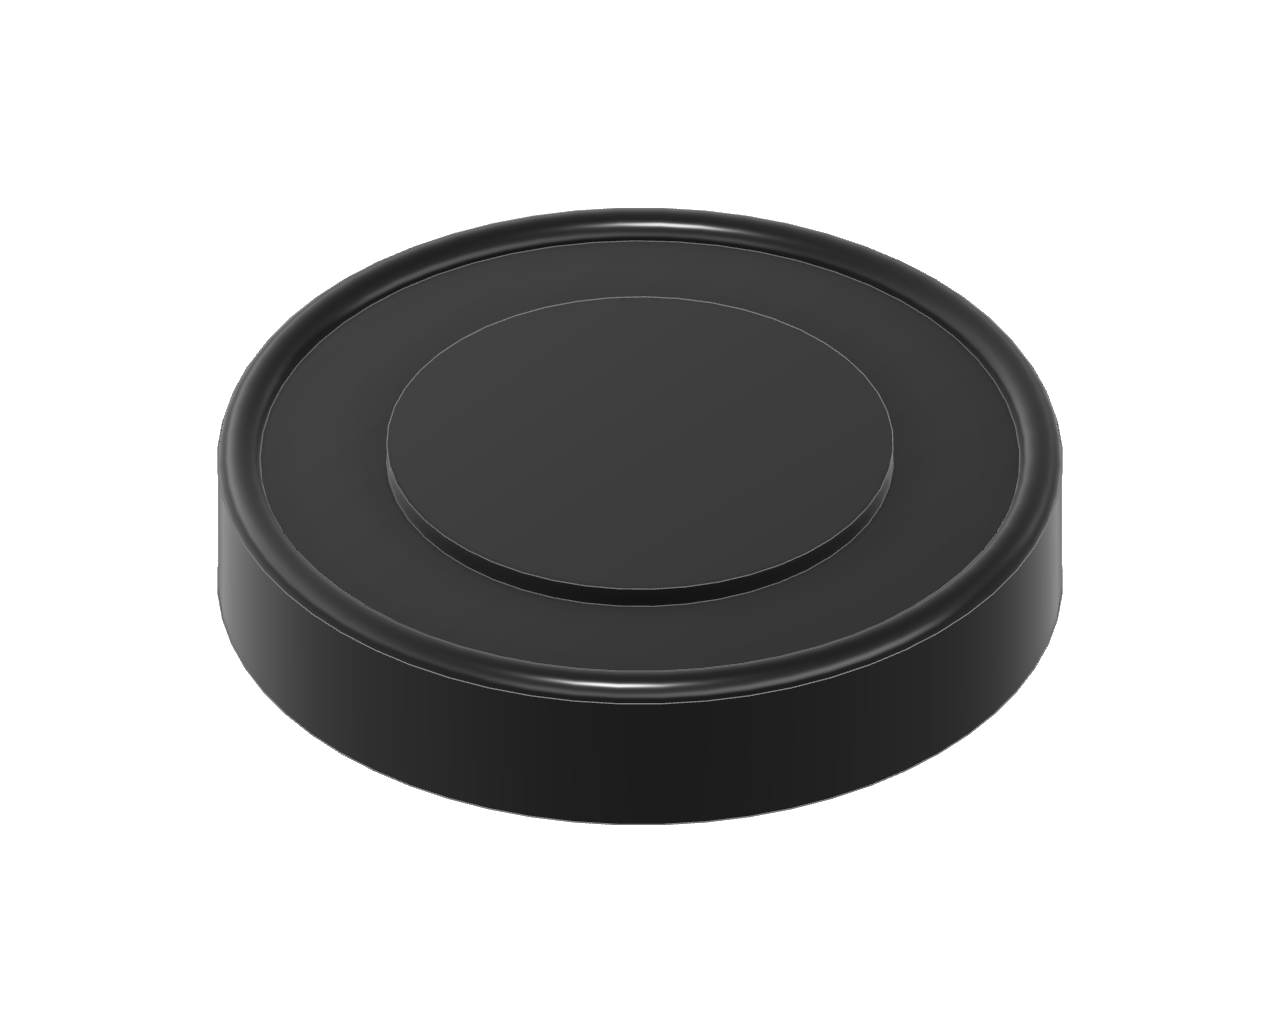
\includegraphics[scale=0.25]{images/process/FlowerLamp.png}
        \caption{Shows a three-dimensional base model of the blossom lamp idea.}
        \label{fig:blossomBaseModel}
        \vspace{6mm}
        \end{subfigure}
        %\hfill
        \hspace{1mm}
        \begin{subfigure}{.45\textwidth}
            \centering
            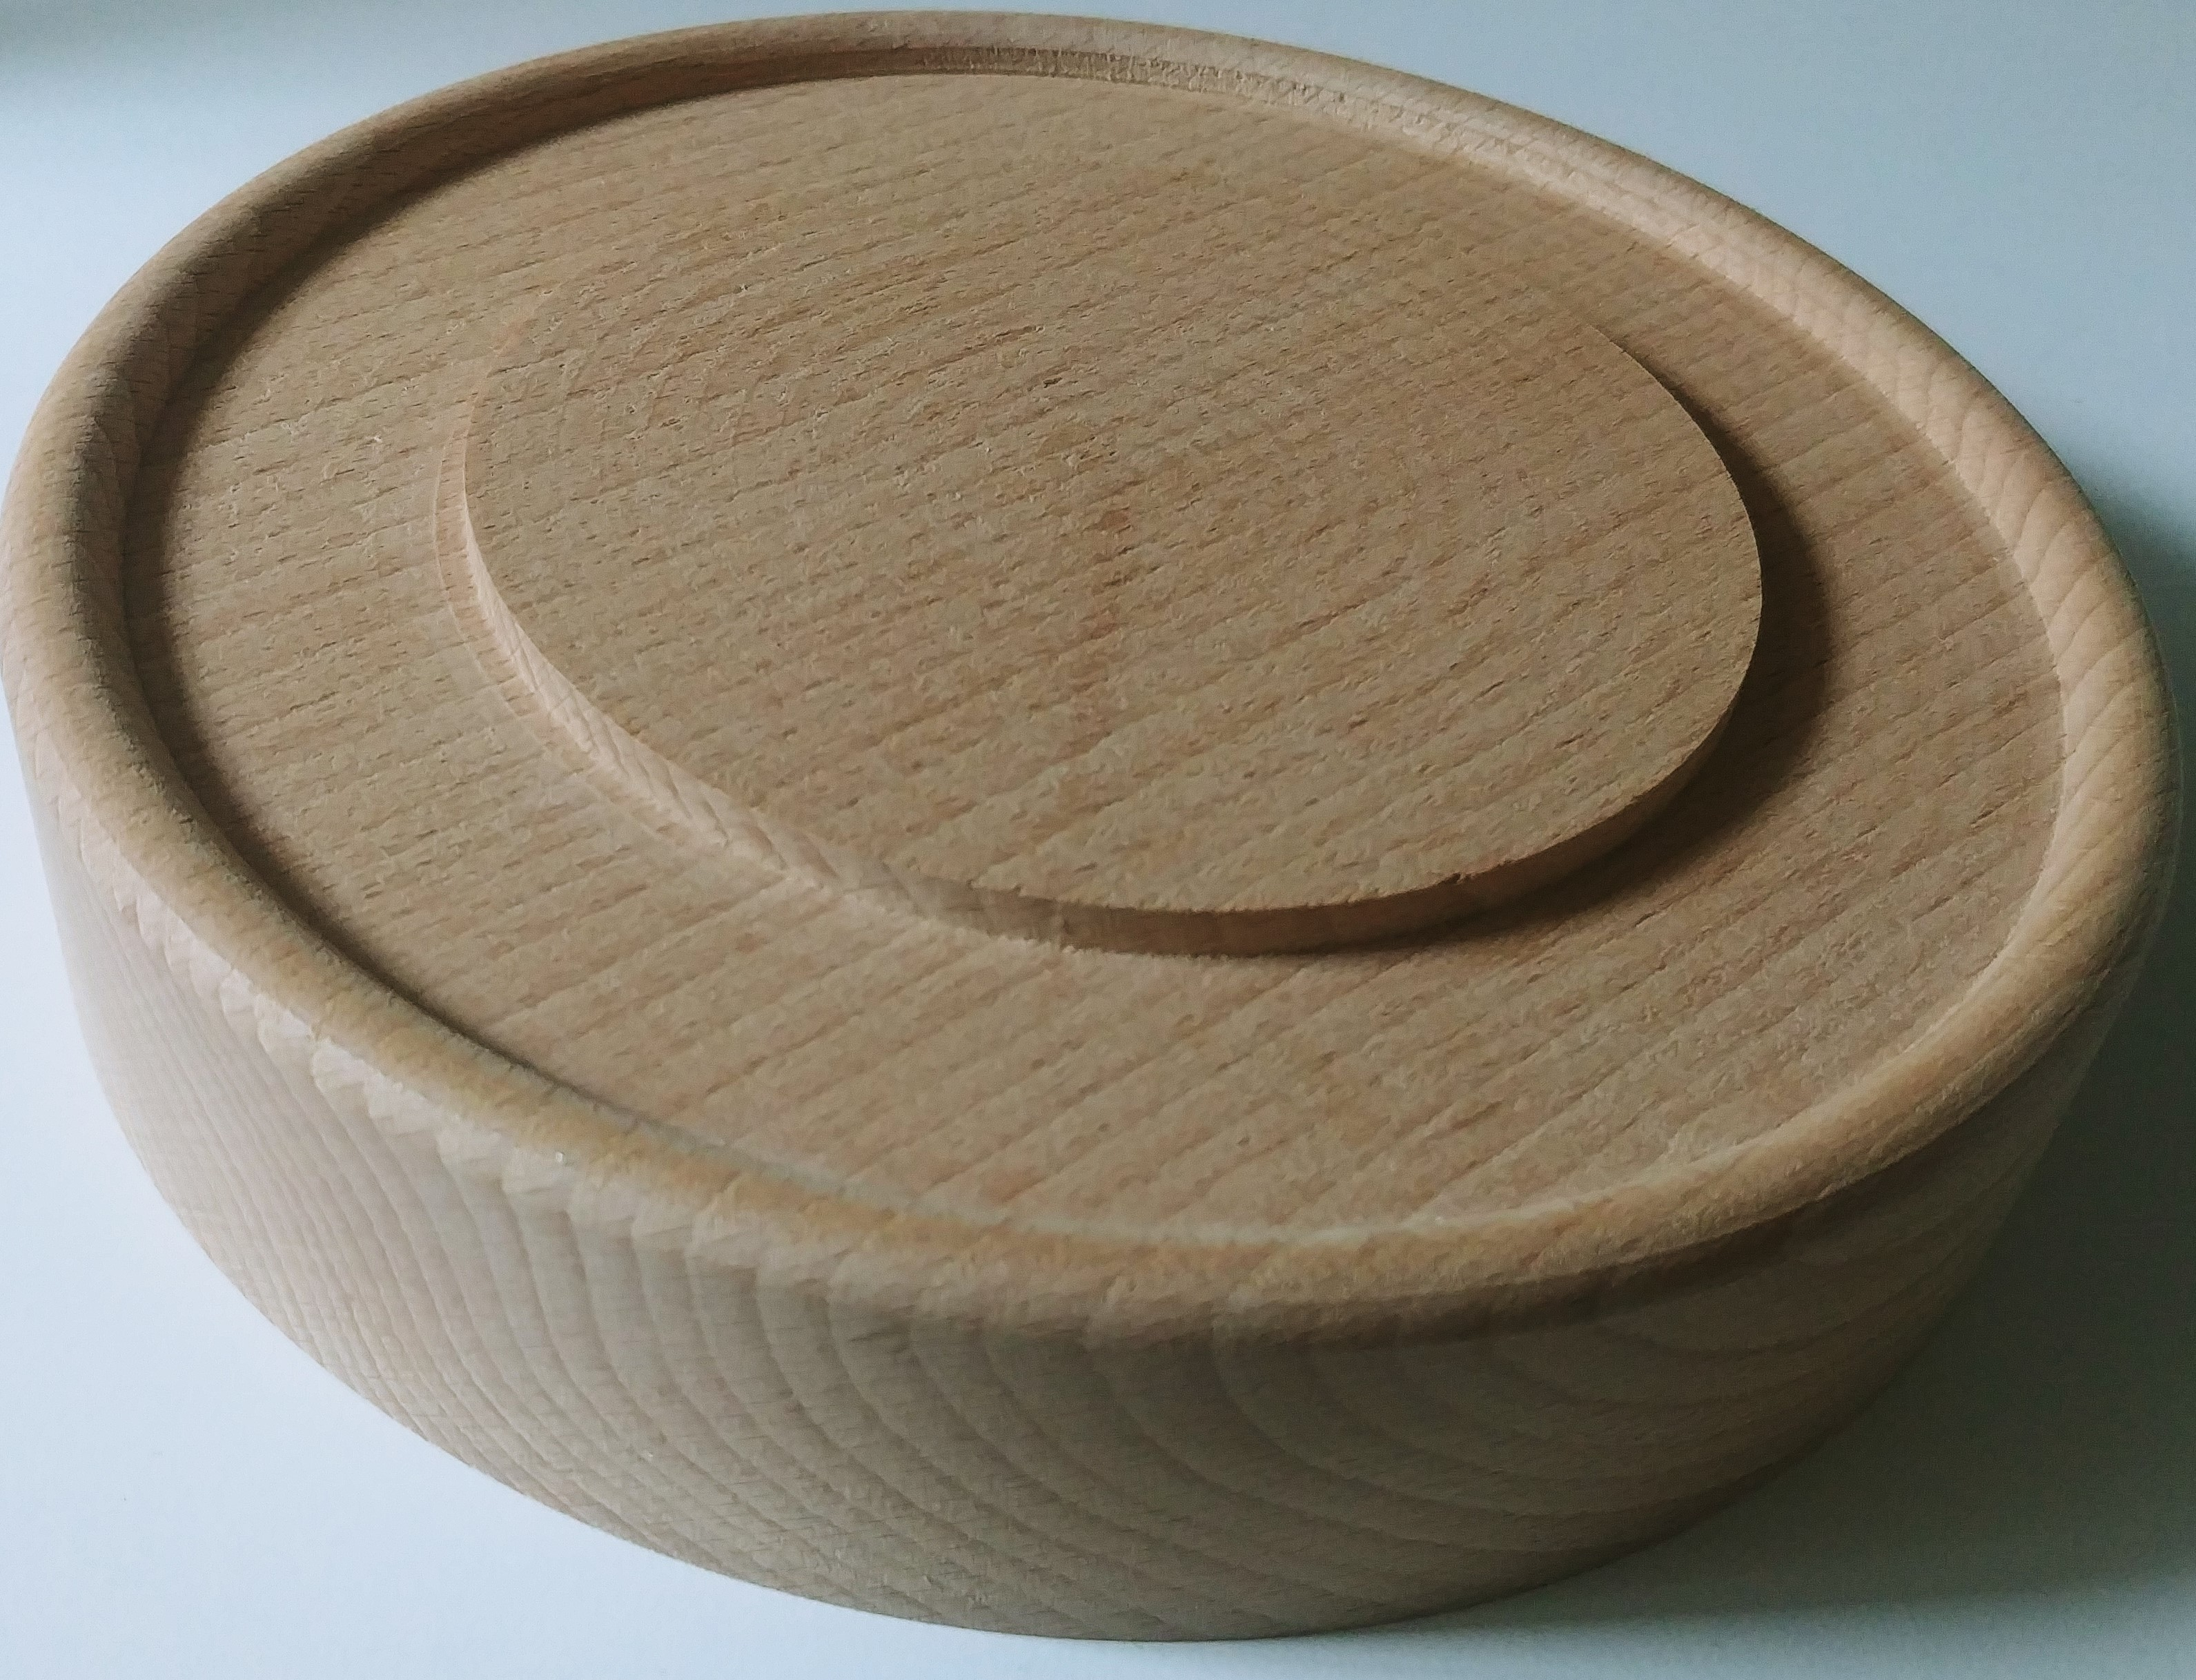
\includegraphics[scale=0.05]{images/process/base.jpg}
            \caption{Shows the base that has been milled.}
            \label{fig:blossomBase}
            \vspace{6mm}
        \end{subfigure}
        %\hfill
        \caption{Show the steps we had to do to drill the base in a CNC machine.}
        \label{fig:laserCutTests}
    \end{figure}


    \noindent
    After milling the base, we had to experiment with a lase cuter to find out how big the holes and the distance between them 
    has to be, so that we can laser cut the blossom shape later. To laser cut everything, we used Illustator\cite{illustrator} 
    and a laser cutter. With Illustator we can design the shape that has to be cut. Therefore, we tried different widths (1mm, 
    0.75mm and 0.5mm) and distances (1mm, 0.75mm, 0.5mm). The result can be found in Figure ~\ref{fig:01_LaserCut}.\\
    \noindent
    After doing the first tried we decided to work with wood because it is more flexible 
    than acrylic glas (see Figure ~\ref{fig:03_LaserCut} and ~\ref{fig:04_LaserCut}).

    \begin{figure}[H]
        \centering
        \begin{subfigure}{.45\textwidth}
        \centering
        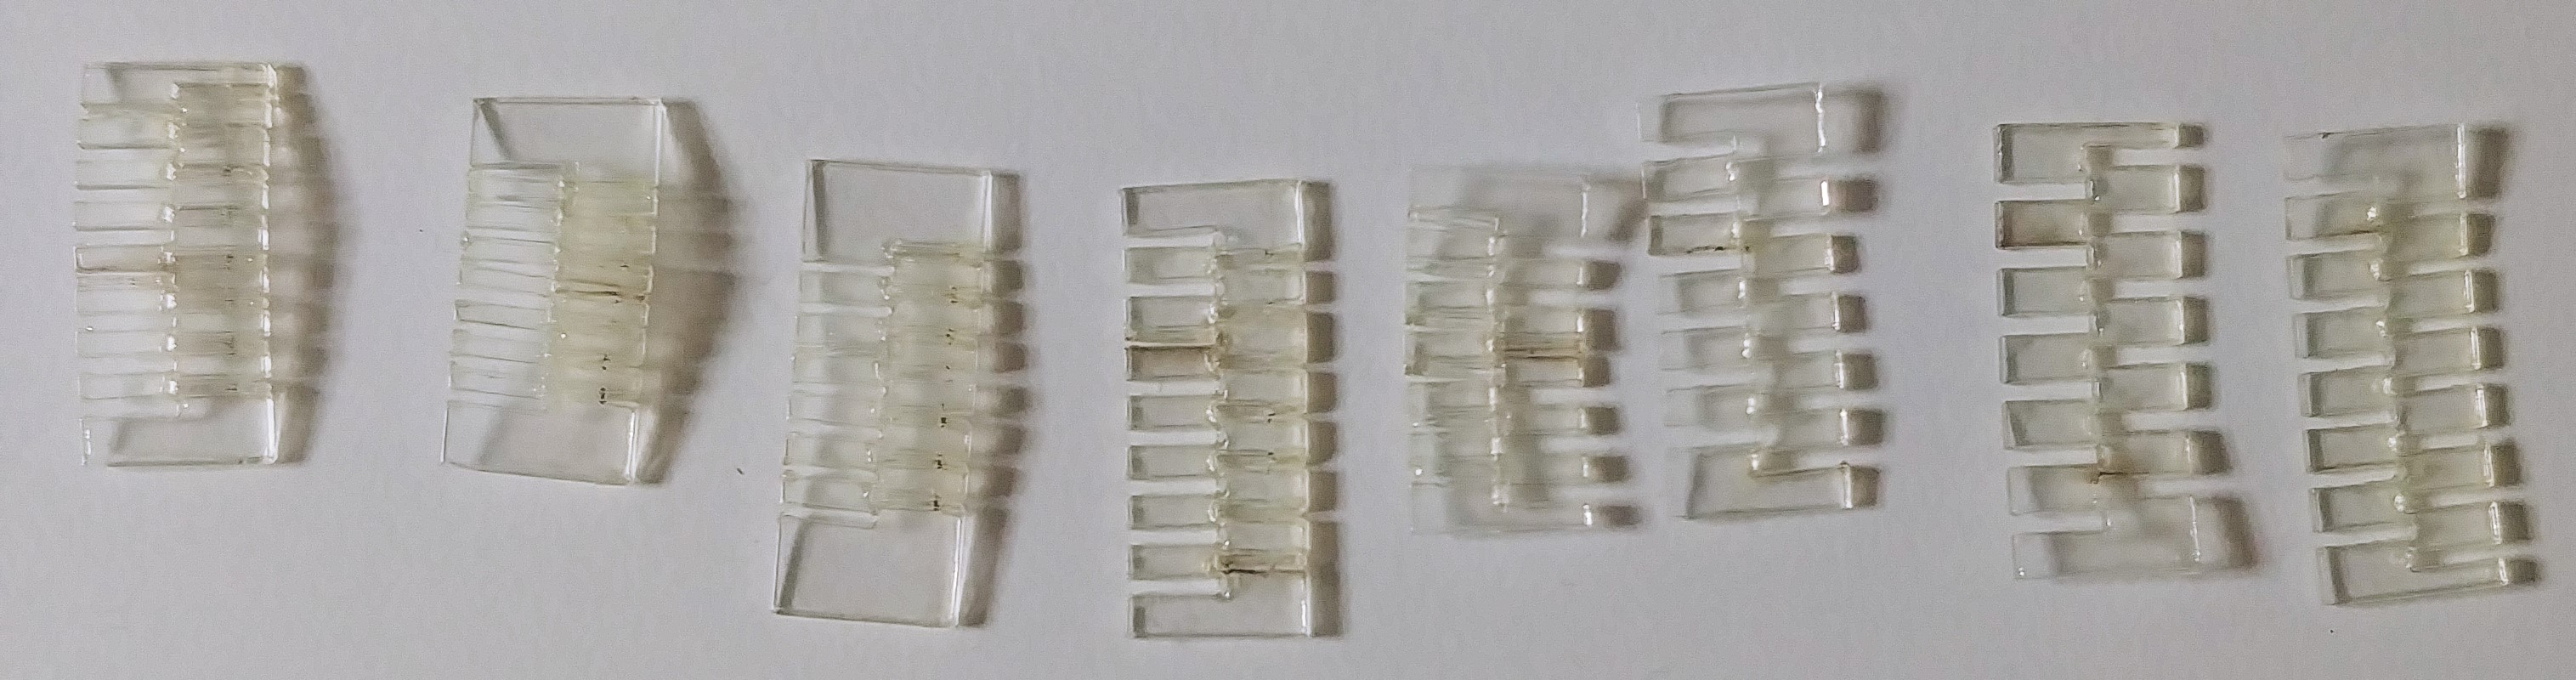
\includegraphics[width=0.8\linewidth]{images/process/01_LaserCut.jpg}
        \caption{Shows the first try to laser cut in general, so we wanted to
                find out what distances of the wholes and how big the wholes 
                should be in general.}
        \label{fig:01_LaserCut}
        \vspace{6mm}
        \end{subfigure}
        %\hfill
        \medskip
        \hspace{1mm}
        \begin{subfigure}{.45\textwidth}
            \centering
            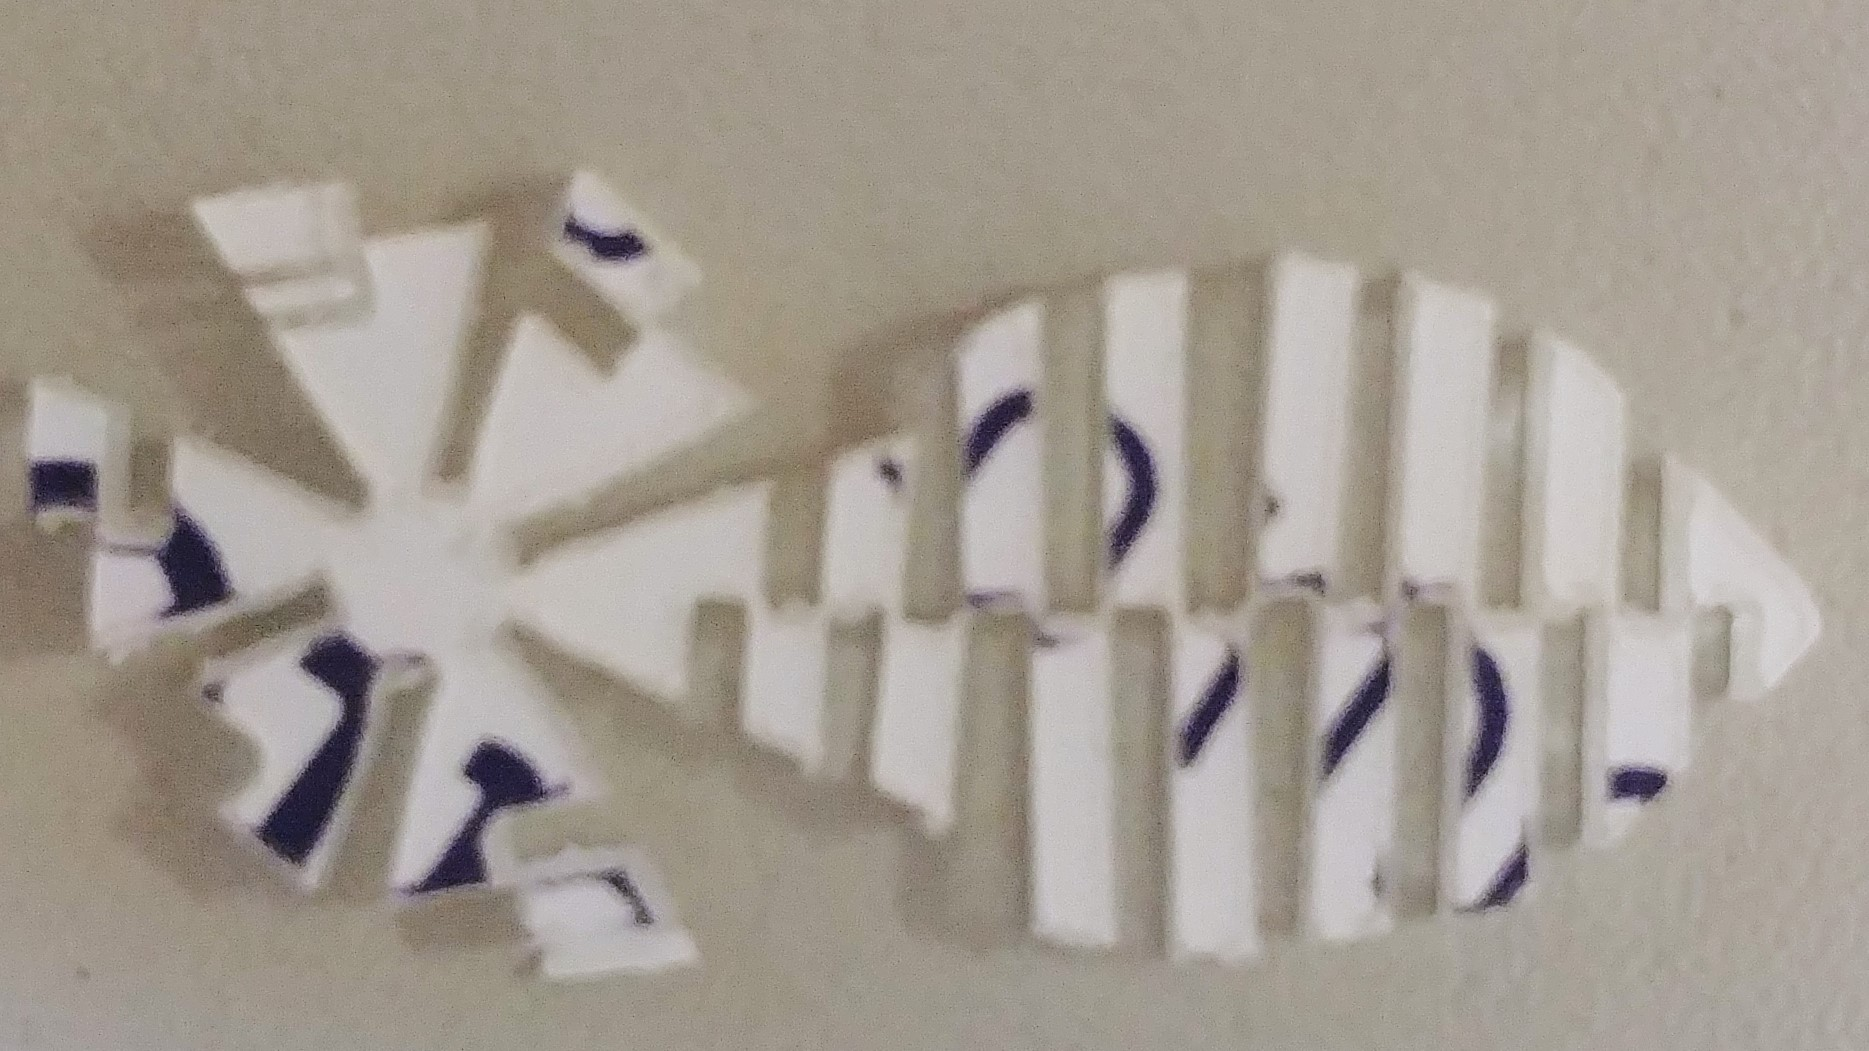
\includegraphics[width=0.6\linewidth]{images/process/02_LaserCut.jpg}
            \caption{Shows the second try to laser cut the shape. This time we have been
                    working with acrylic glass that was 2mm thin. The wholes are 1mm thick 
                    and the distance between those are only 5mm. When we tried to move
                    the parts, they broke.}
            \label{fig:02_LaserCut}
            \vspace{6mm}
        \end{subfigure}
        %\hfill
        \hspace{1mm}
        \begin{subfigure}{.45\textwidth}
            \centering
            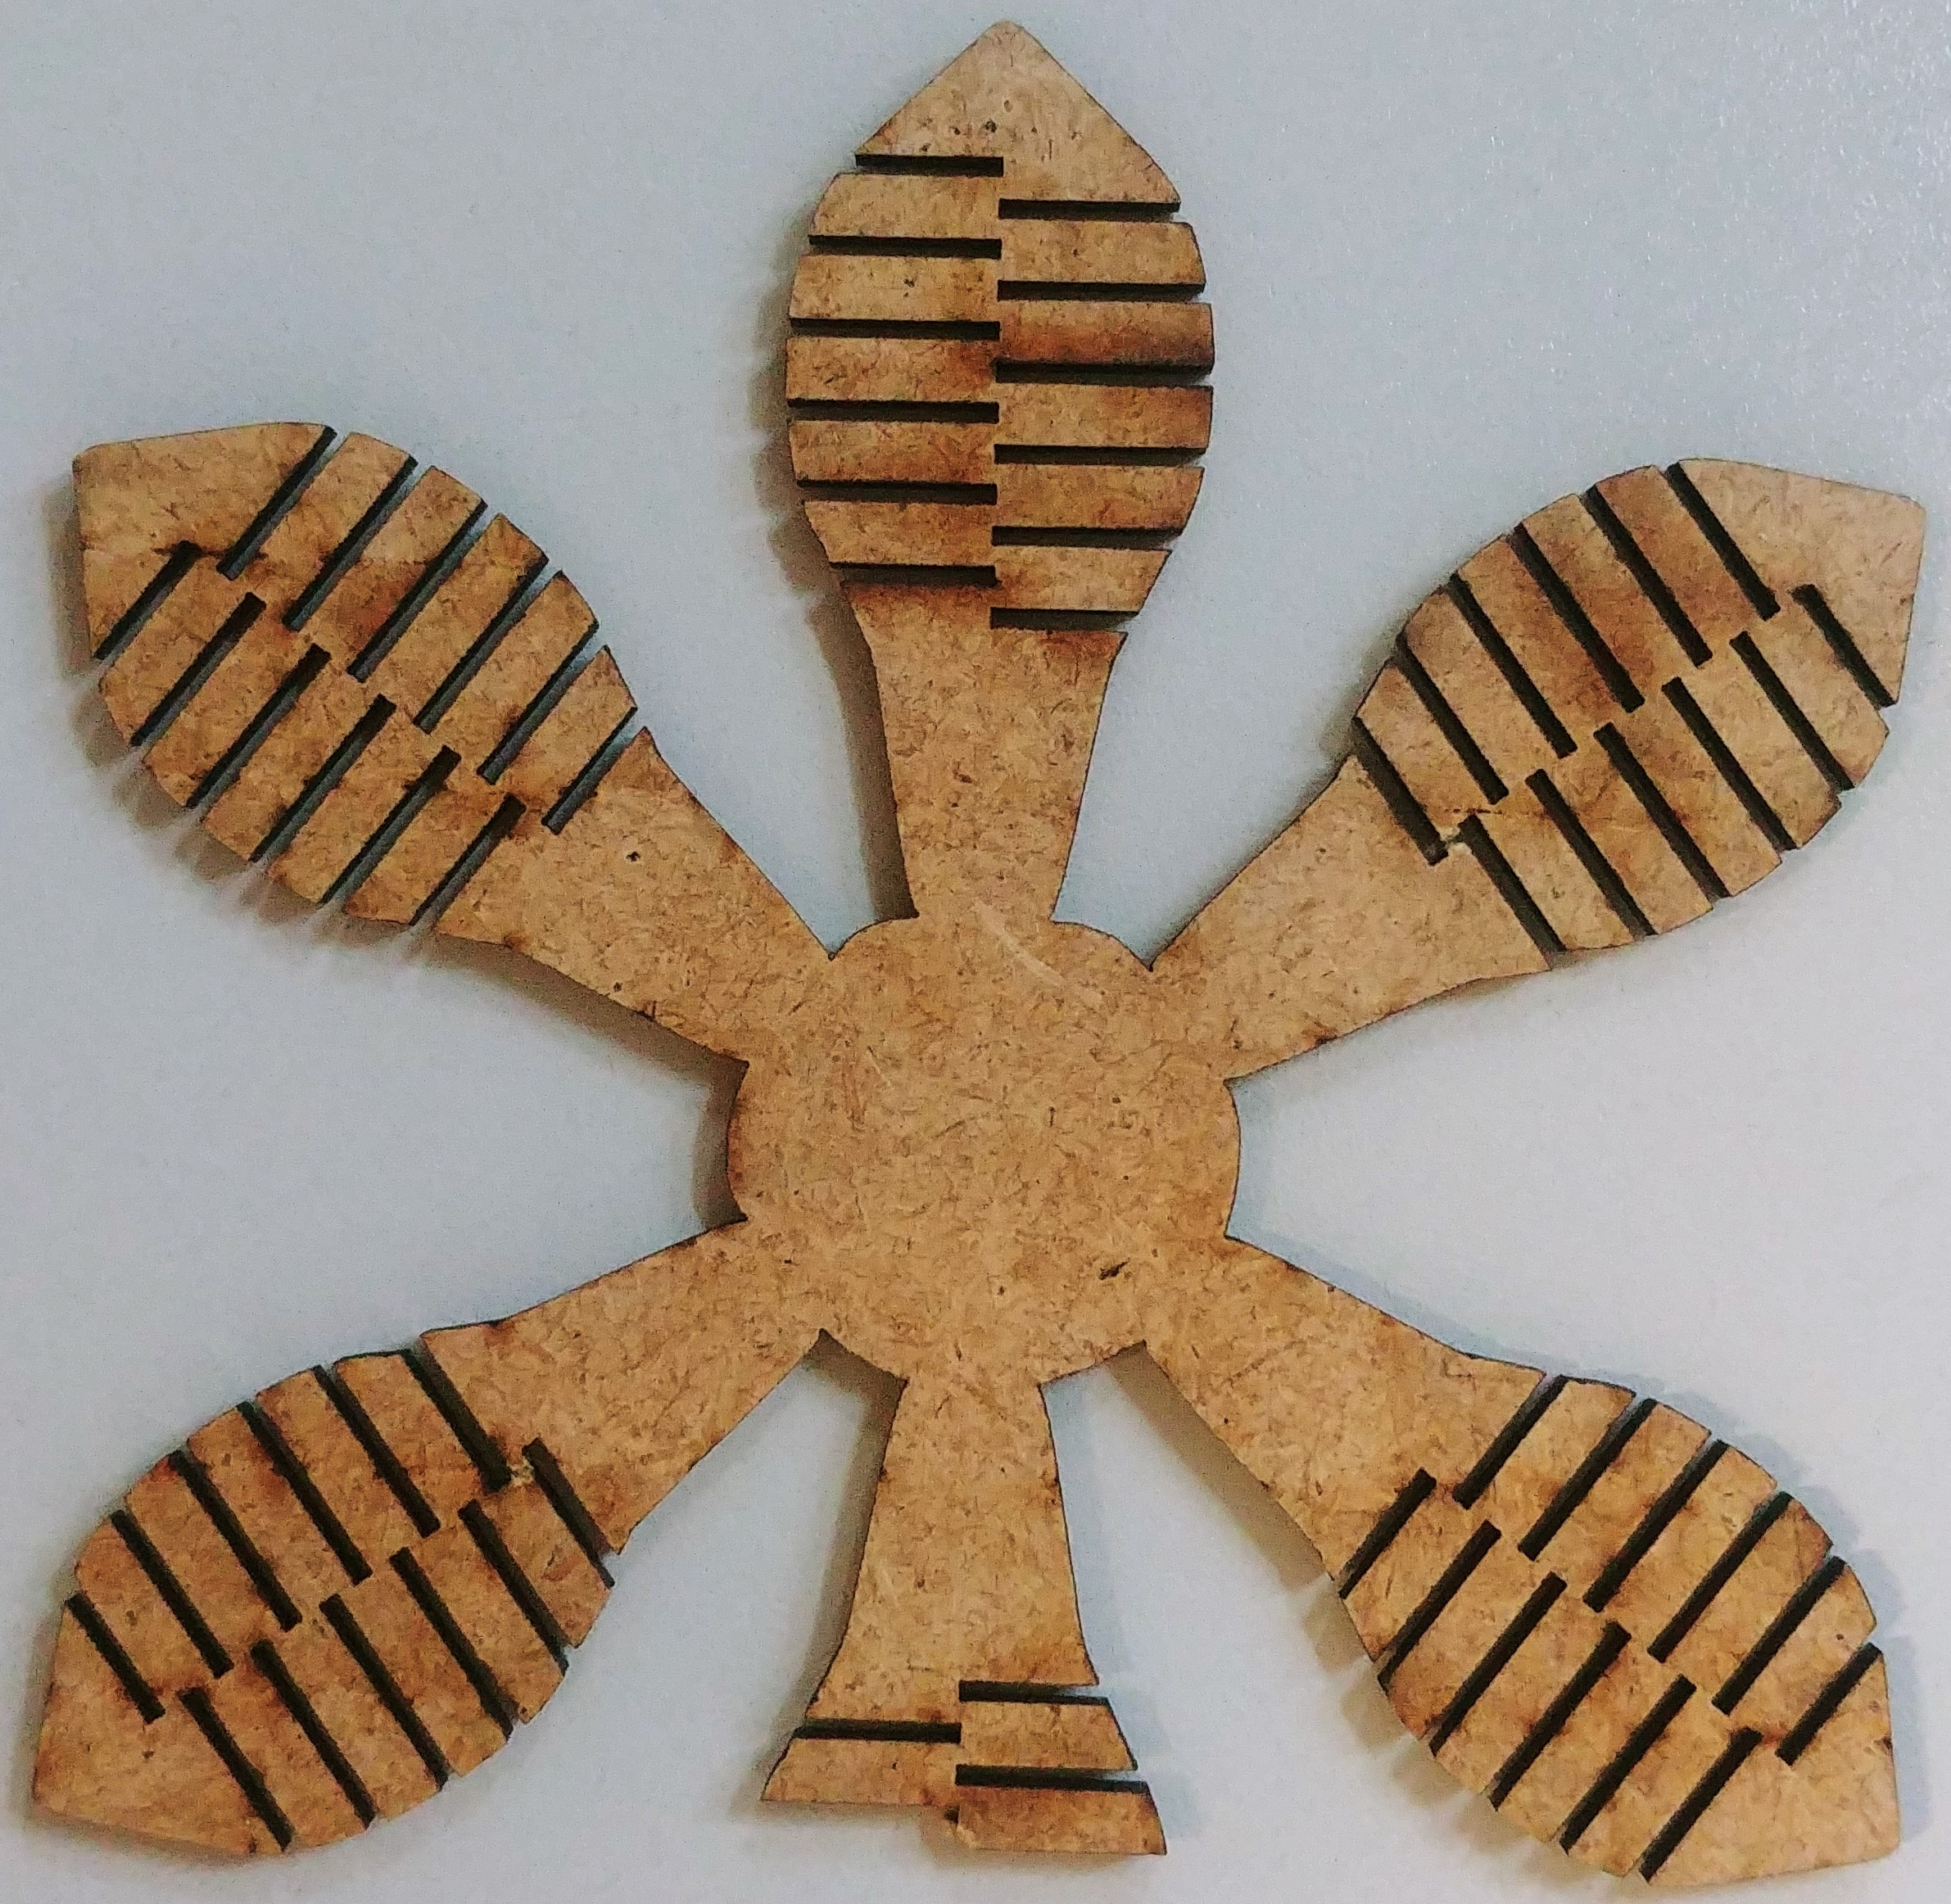
\includegraphics[width=0.6\linewidth]{images/process/03_LaserCut.jpg}
            \caption{Shows the third try to laser cut the shape. This time we have been
                    working with wood plate what is 3mm thin. The wholes are 1mm thick 
                    and the distance between those are only 5mm. When we tried to move
                    the parts, they broke.}
            \label{fig:03_LaserCut}
            \vspace{6mm}
        \end{subfigure}
        %\hfill
        \hspace{1mm}
        \begin{subfigure}{.45\textwidth}
            \centering
            \includegraphics[width=0.6\linewidth]{images/process/04_LaserCut.jpg}
            \caption{Shows the fourth try to laser cut the shape. This time we have been
                    working with MDR 1mm thin plate. The wholes are 0.5mm thick and the 
                    distance between those are only 2.5mm, so they broke.}
            \label{fig:04_LaserCut}
            \vspace{6mm}
        \end{subfigure}
        \hspace{1mm}
        \begin{subfigure}{.45\textwidth}
            \centering
            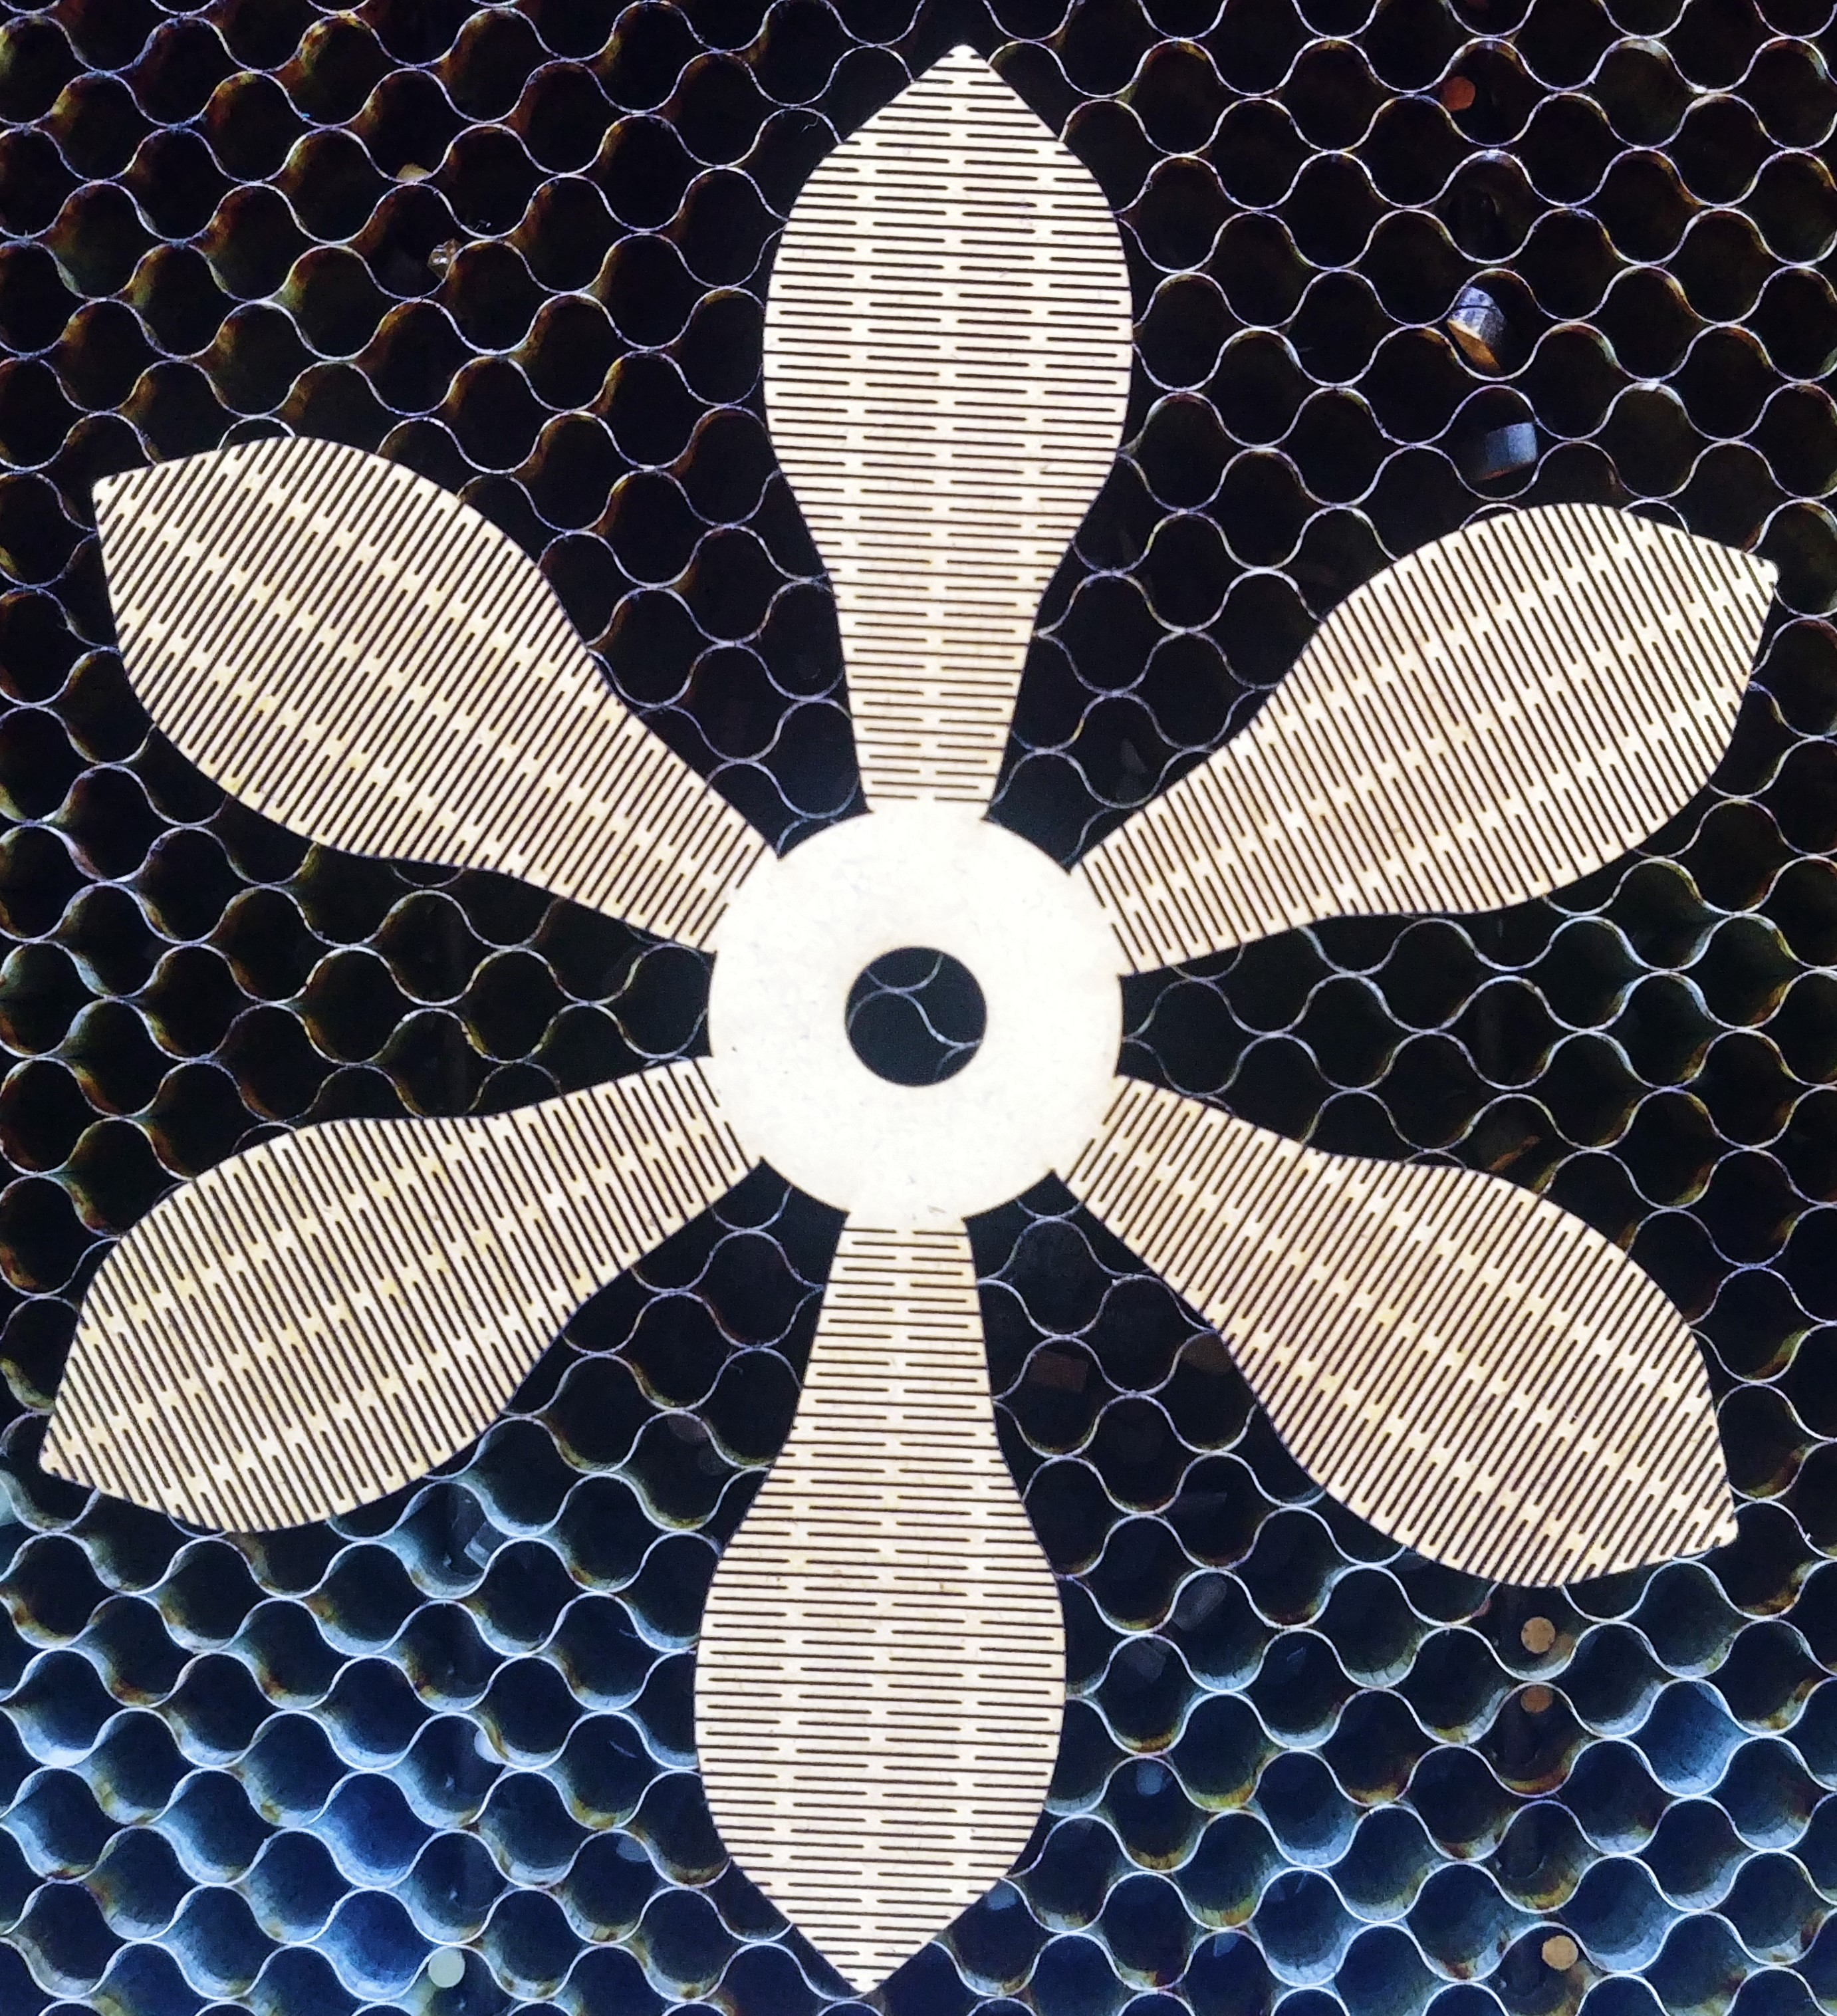
\includegraphics[width=0.6\linewidth]{images/process/05_LaserCut.jpg}
            \caption{Shows the fifth try to laser cut the shape. This time we have been
                    working with MDR 1mm thin plate. They wholes are just lines. Nothines
                    broke and it is truely flexible. \cite{Festi2016}}
            \label{fig:04_LaserCut}
            \vspace{6mm}
        \end{subfigure}
        \hspace{1mm}
        \begin{subfigure}{.45\textwidth}
            \centering
            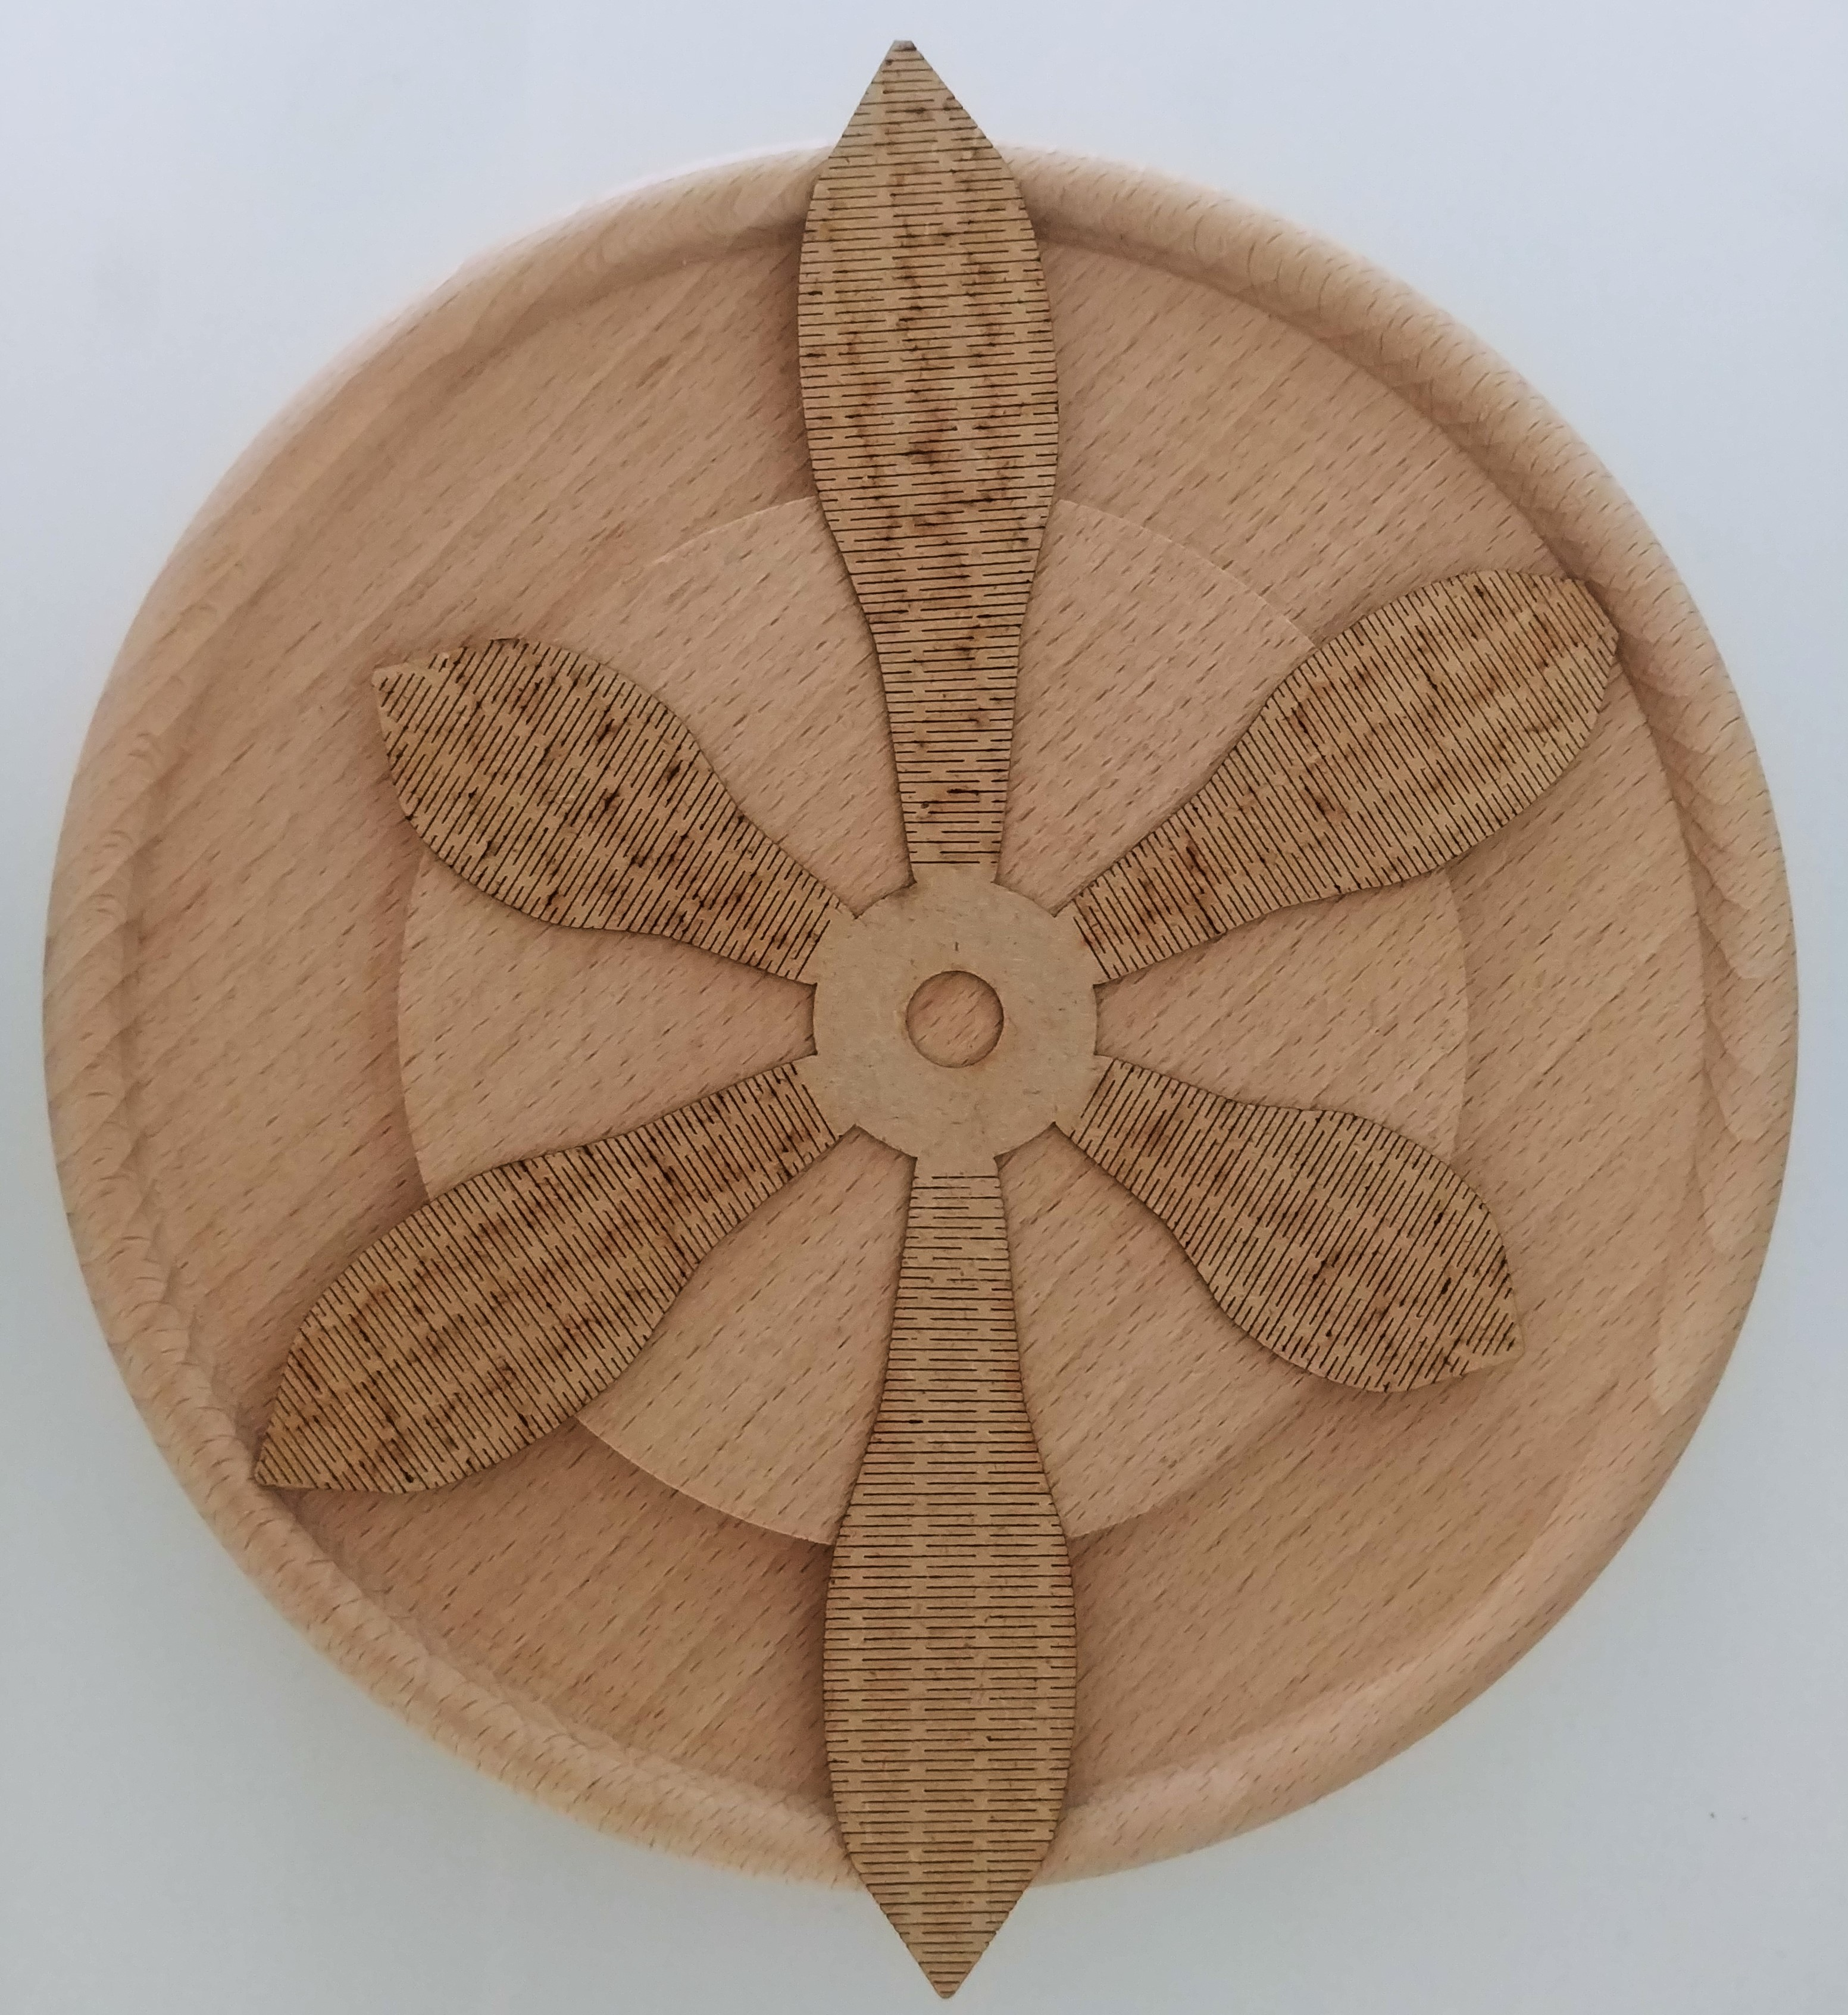
\includegraphics[width=0.6\linewidth]{images/process/06_LaserCut.jpg}
            \caption{Shows the sixth and last try to laser cut the shape. Everything is 
            working now, so the wood is flexable and the blossoms leaves are long enough
            to connect. }
            \label{fig:04_LaserCut}
            \vspace{6mm}
        \end{subfigure}
        \caption{Shows the process of laser cuttings.}
        \label{fig:laserCutTests}
    \end{figure}

    \noindent
    In addition to this, we tested the conductive ink on the wood and if it is possible 
    to get a connection between to leaves if they have conductive ink on it. The result is
    that it is possible to get a notification; however, the resistance is very high, so we 
    had to use an analog pin and a threshold to find out if a leave coupe is connected
    (see \ref{fig:leaveConductiveInk}).

    \begin{figure}[h!]
        \centering
        \includegraphics[scale=0.05]{images/process/leaveTesting.jpg}
        \caption{Shows the testing of the conductive ink with wooden leaves.}
        \label{fig:leaveConductiveInk}
    \end{figure}

    \noindent
    Furthermore, we used a vinyl cutter to cut our cupper foil in a round shape. This copper foil 
    tags will be used as capacitive sensors. These will be used as sliders in the program, so the 
    user can change the brightness of the LEDs (see Figure \ref{fig:vinylCuttingProp}).

    \begin{figure}[h!]
        \centering
        \includegraphics[scale=0.05]{images/process/vinylCuttingProp.jpg}
        \caption{Shows the vinyl cutting result.}
        \label{fig:vinylCuttingProp}
    \end{figure}

    \noindent
    Afterward the conductive test (see Figure \ref{fig:leaveConductiveInk}), we wanted to paint 
    conductive ink on wood before laser cutting. Before, we asked the company if there is 
    something inside the paint that burns or is toxic. After knowing that it should be fine to 
    use the paint and later cut it, we did so (see Figure \ref{fig:leaveConductiveInk_laserCut}). 

    \begin{figure}[h!]
        \centering
        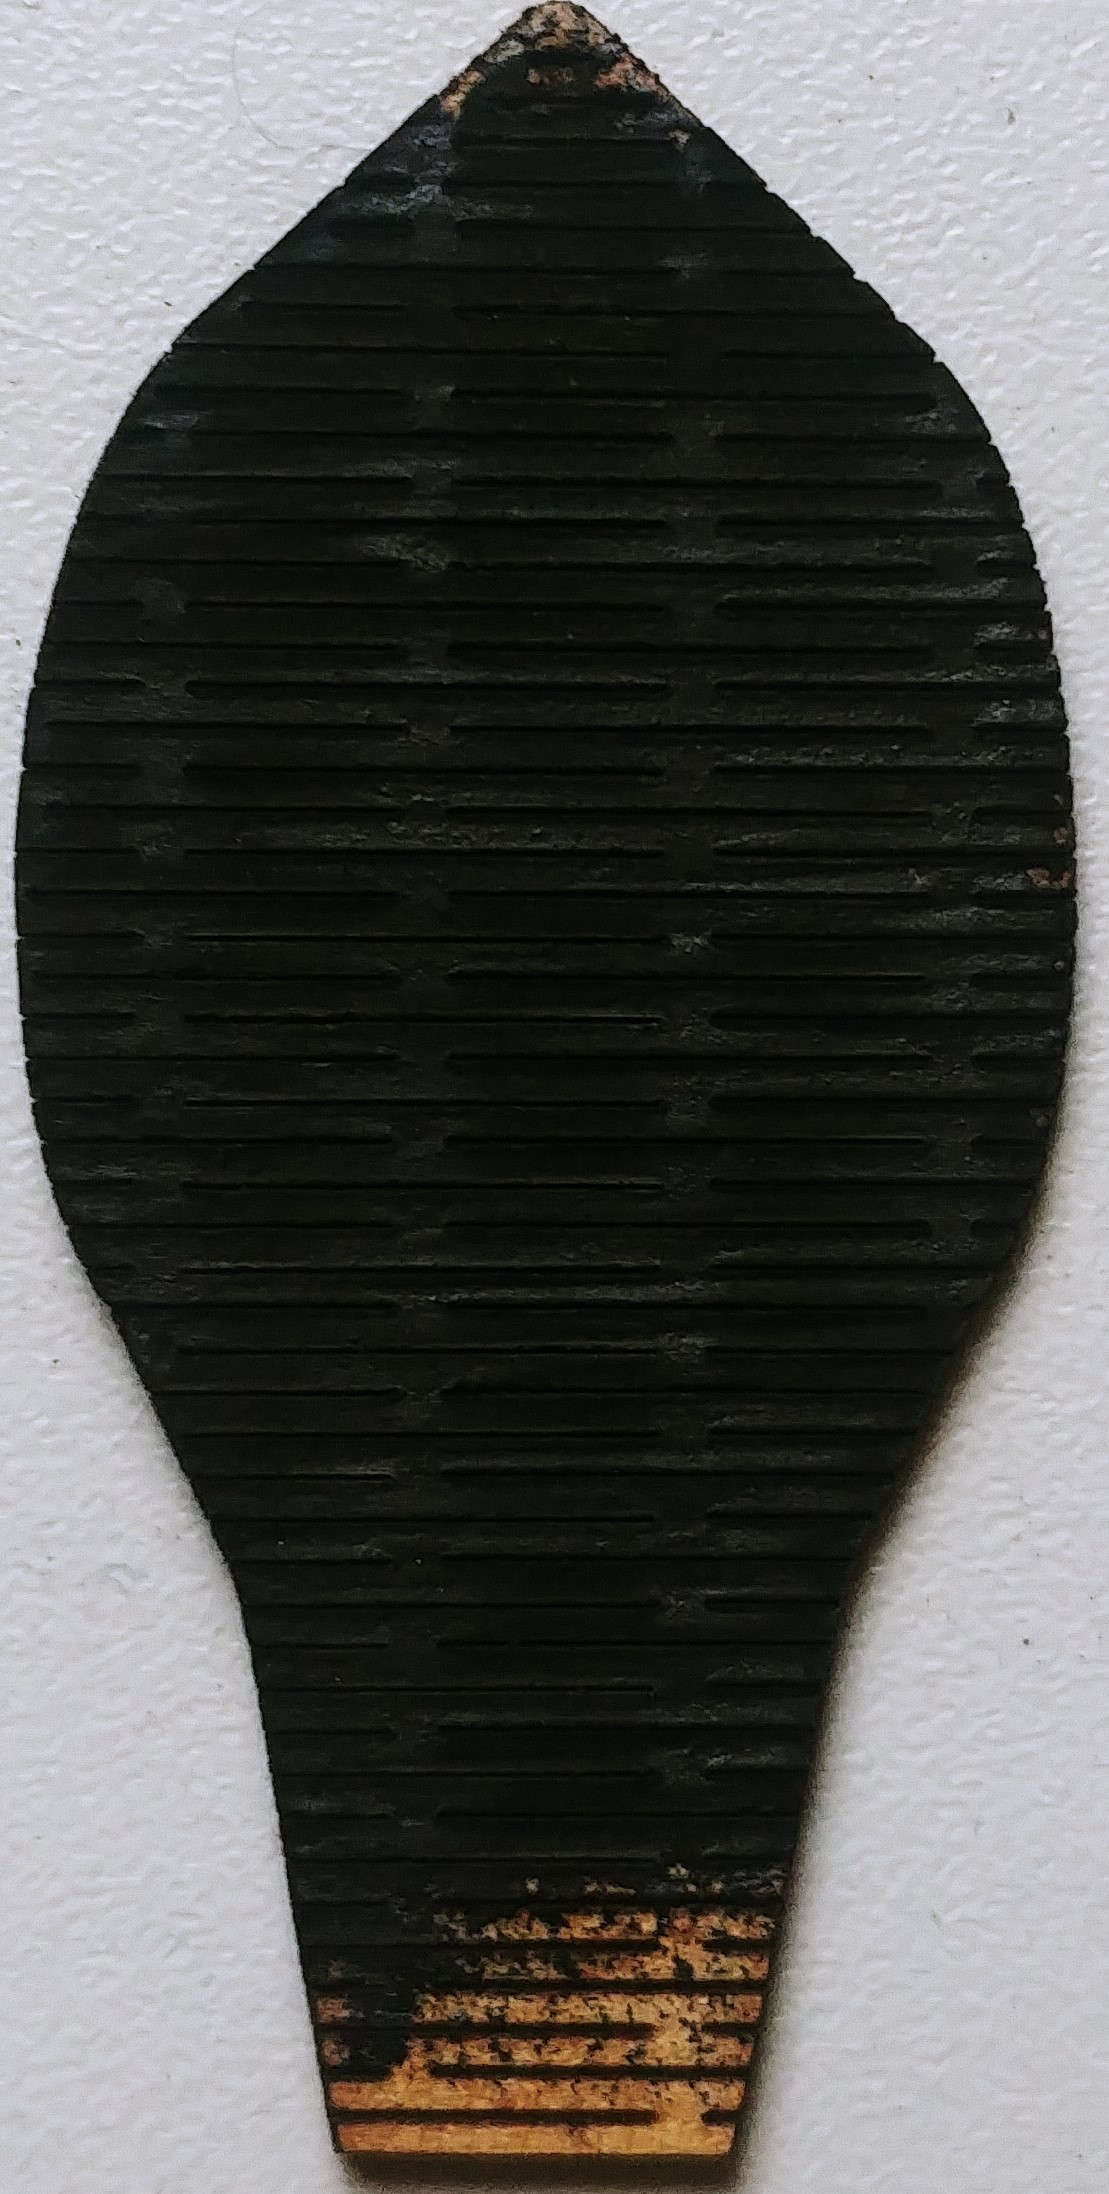
\includegraphics[scale=0.05]{images/process/leaveConductiveInk_laserCut.jpg}
        \caption{Shows a test if conductive ink can be painted on wood before laser cutting it.}
        \label{fig:leaveConductiveInk_laserCut}
    \end{figure}

    \noindent
    Afterwards, we had to drill holes inside the base, so we can link the conductive cupper foil 
    with wires (see \ref{fig:conductiveCupperFoilWithWires}). In addition to this, we had to 
    drill a larger hole inside the base. In this we want to attach the microcontroller and the 
    battery (see \ref{fig:holesForMicrocontroller}). Furthermore, we drilled paths inside the 
    base, so wires can go from every whole to the microcontroller. So, users should not see 
    any wires outside of the whole installation (see \ref{fig:drillPath}).

    \begin{figure}[H]
        \centering
        \begin{subfigure}{.45\textwidth}
        \centering
        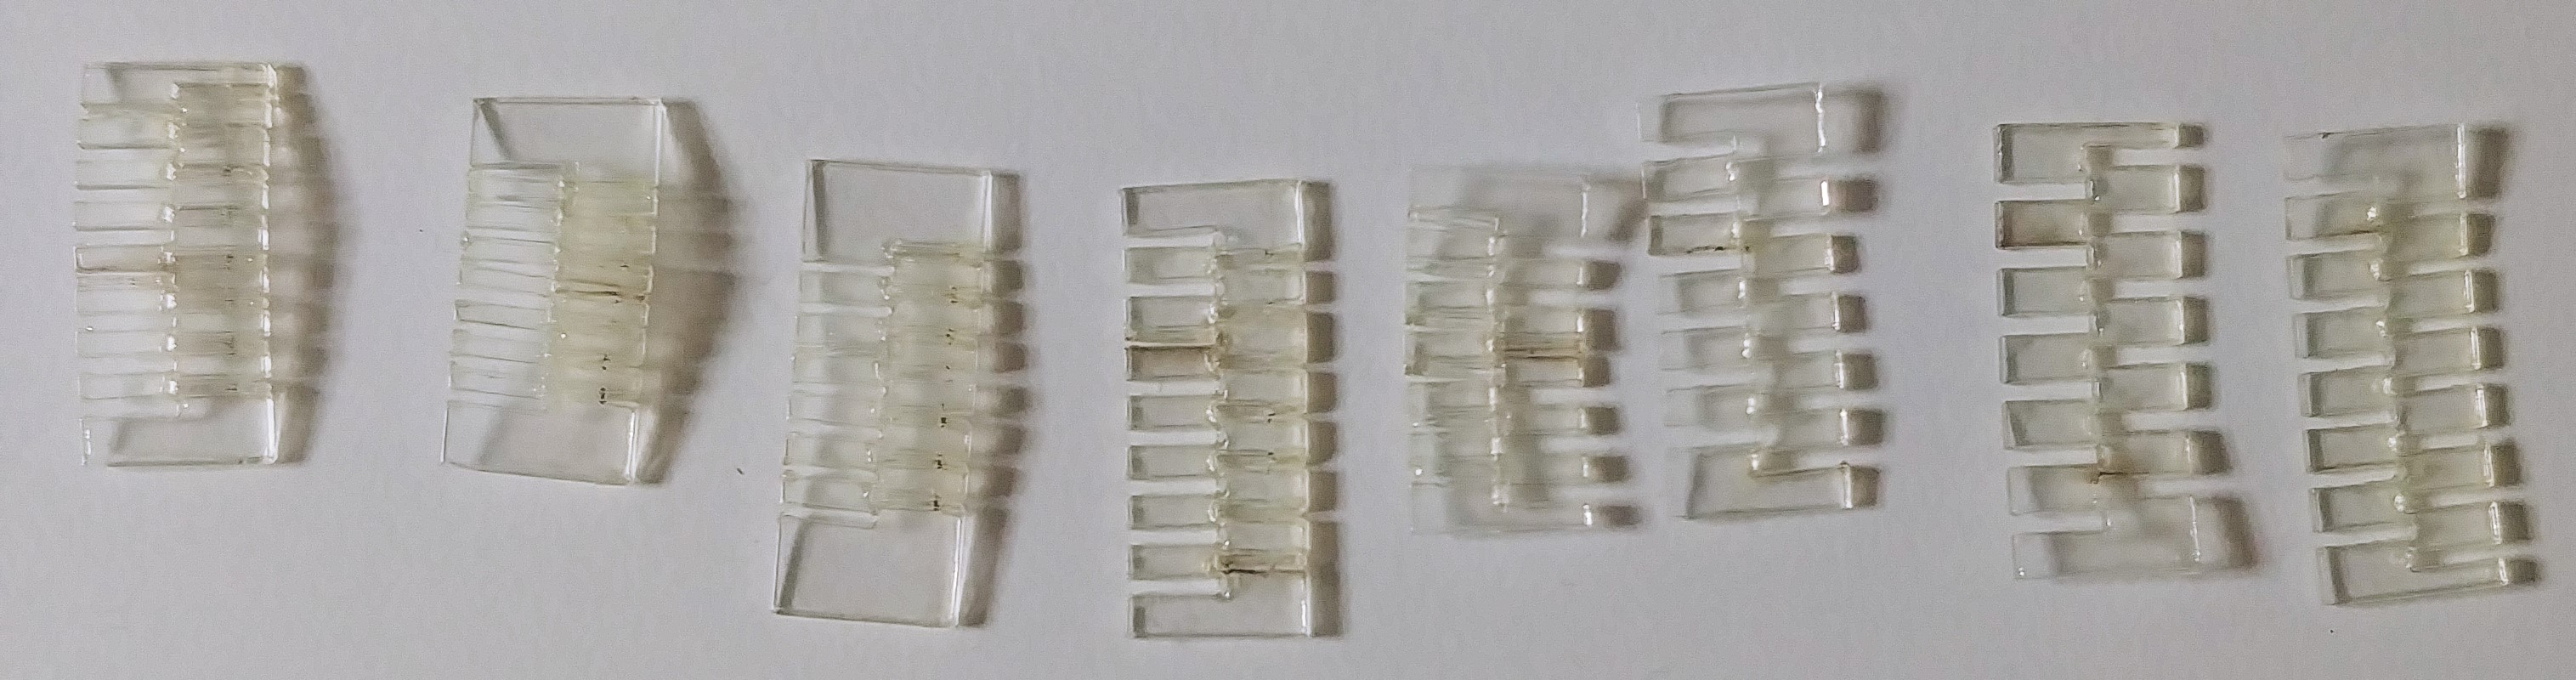
\includegraphics[width=0.8\linewidth]{images/process/01_LaserCut.jpg}
        \caption{Shows the wholes for the cupper foil and their wires.}
        \label{fig:conductiveCupperFoilWithWires}
        \vspace{6mm}
        \end{subfigure}
        %\hfill
        \medskip
        \hspace{1mm}
        \begin{subfigure}{.45\textwidth}
            \centering
            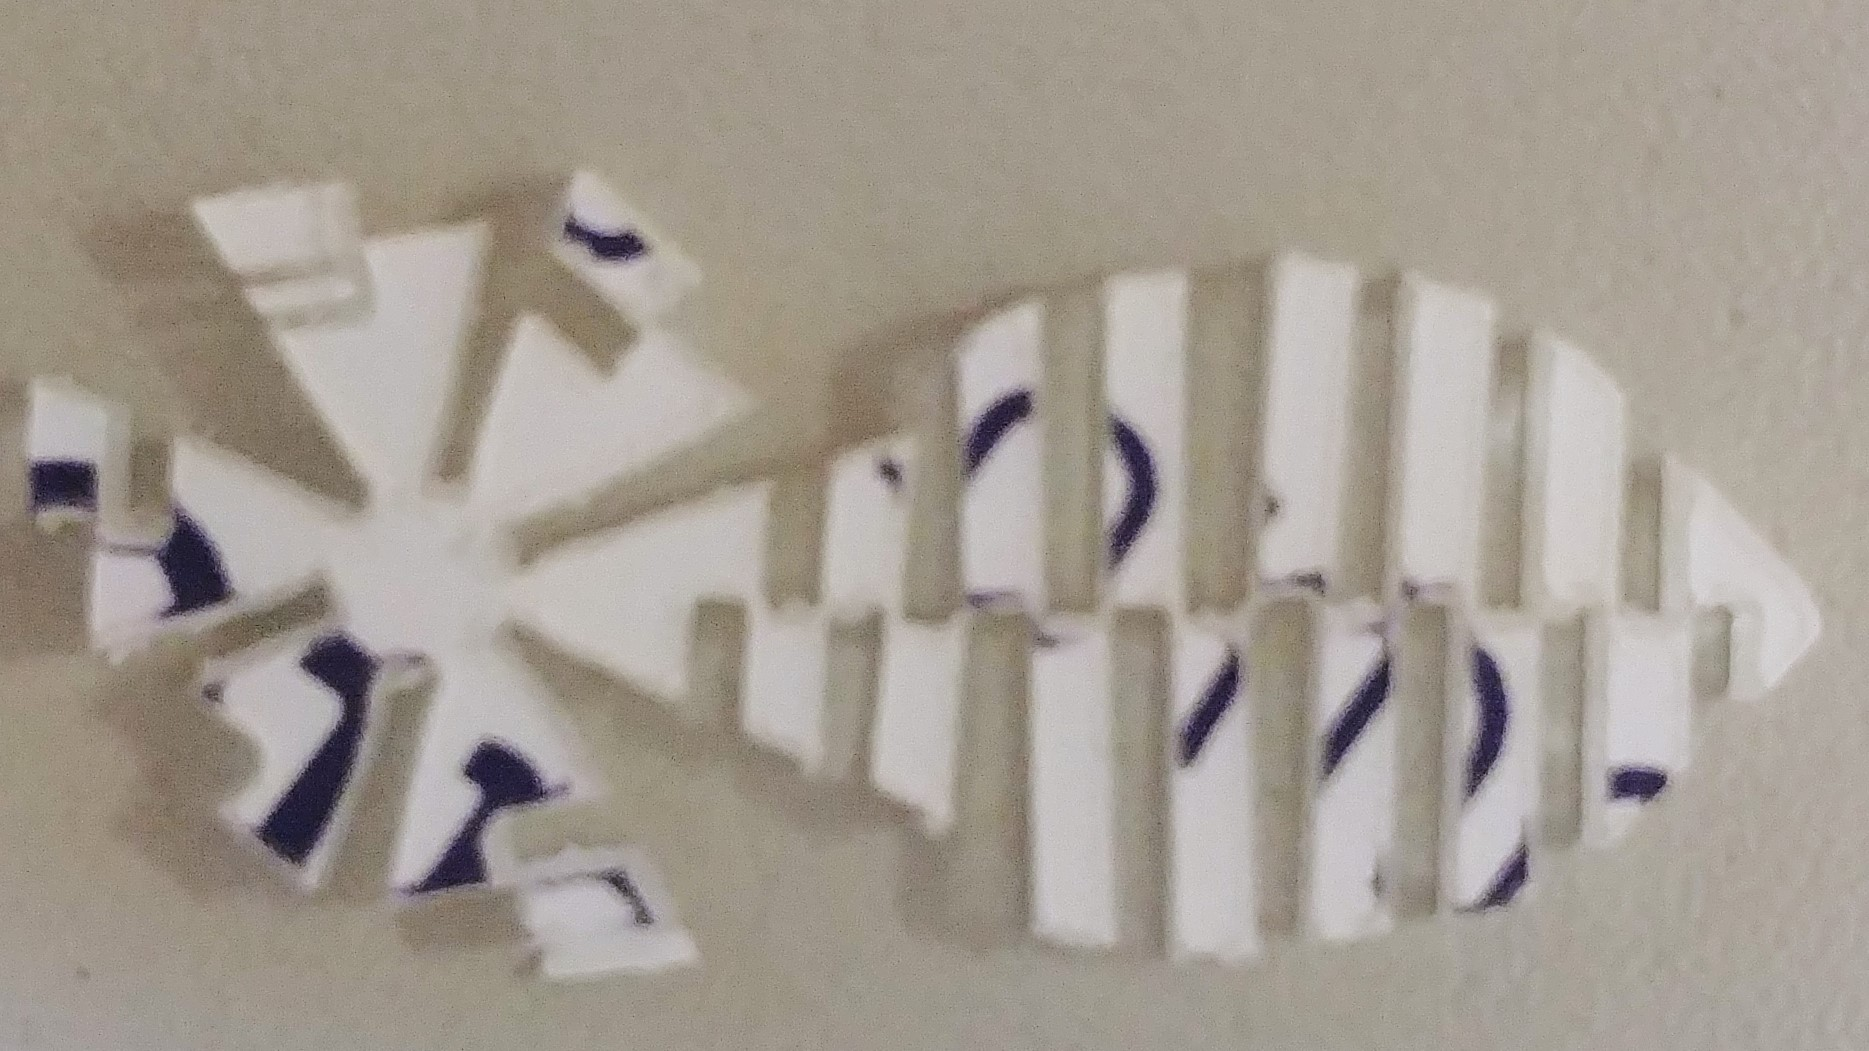
\includegraphics[width=0.6\linewidth]{images/process/02_LaserCut.jpg}
            \caption{Shows the whole where the microcontroller will be attached to.}
            \label{fig:holesForMicrocontroller}
            \vspace{6mm}
        \end{subfigure}
        %\hfill
        \hspace{1mm}
        \begin{subfigure}{.45\textwidth}
            \centering
            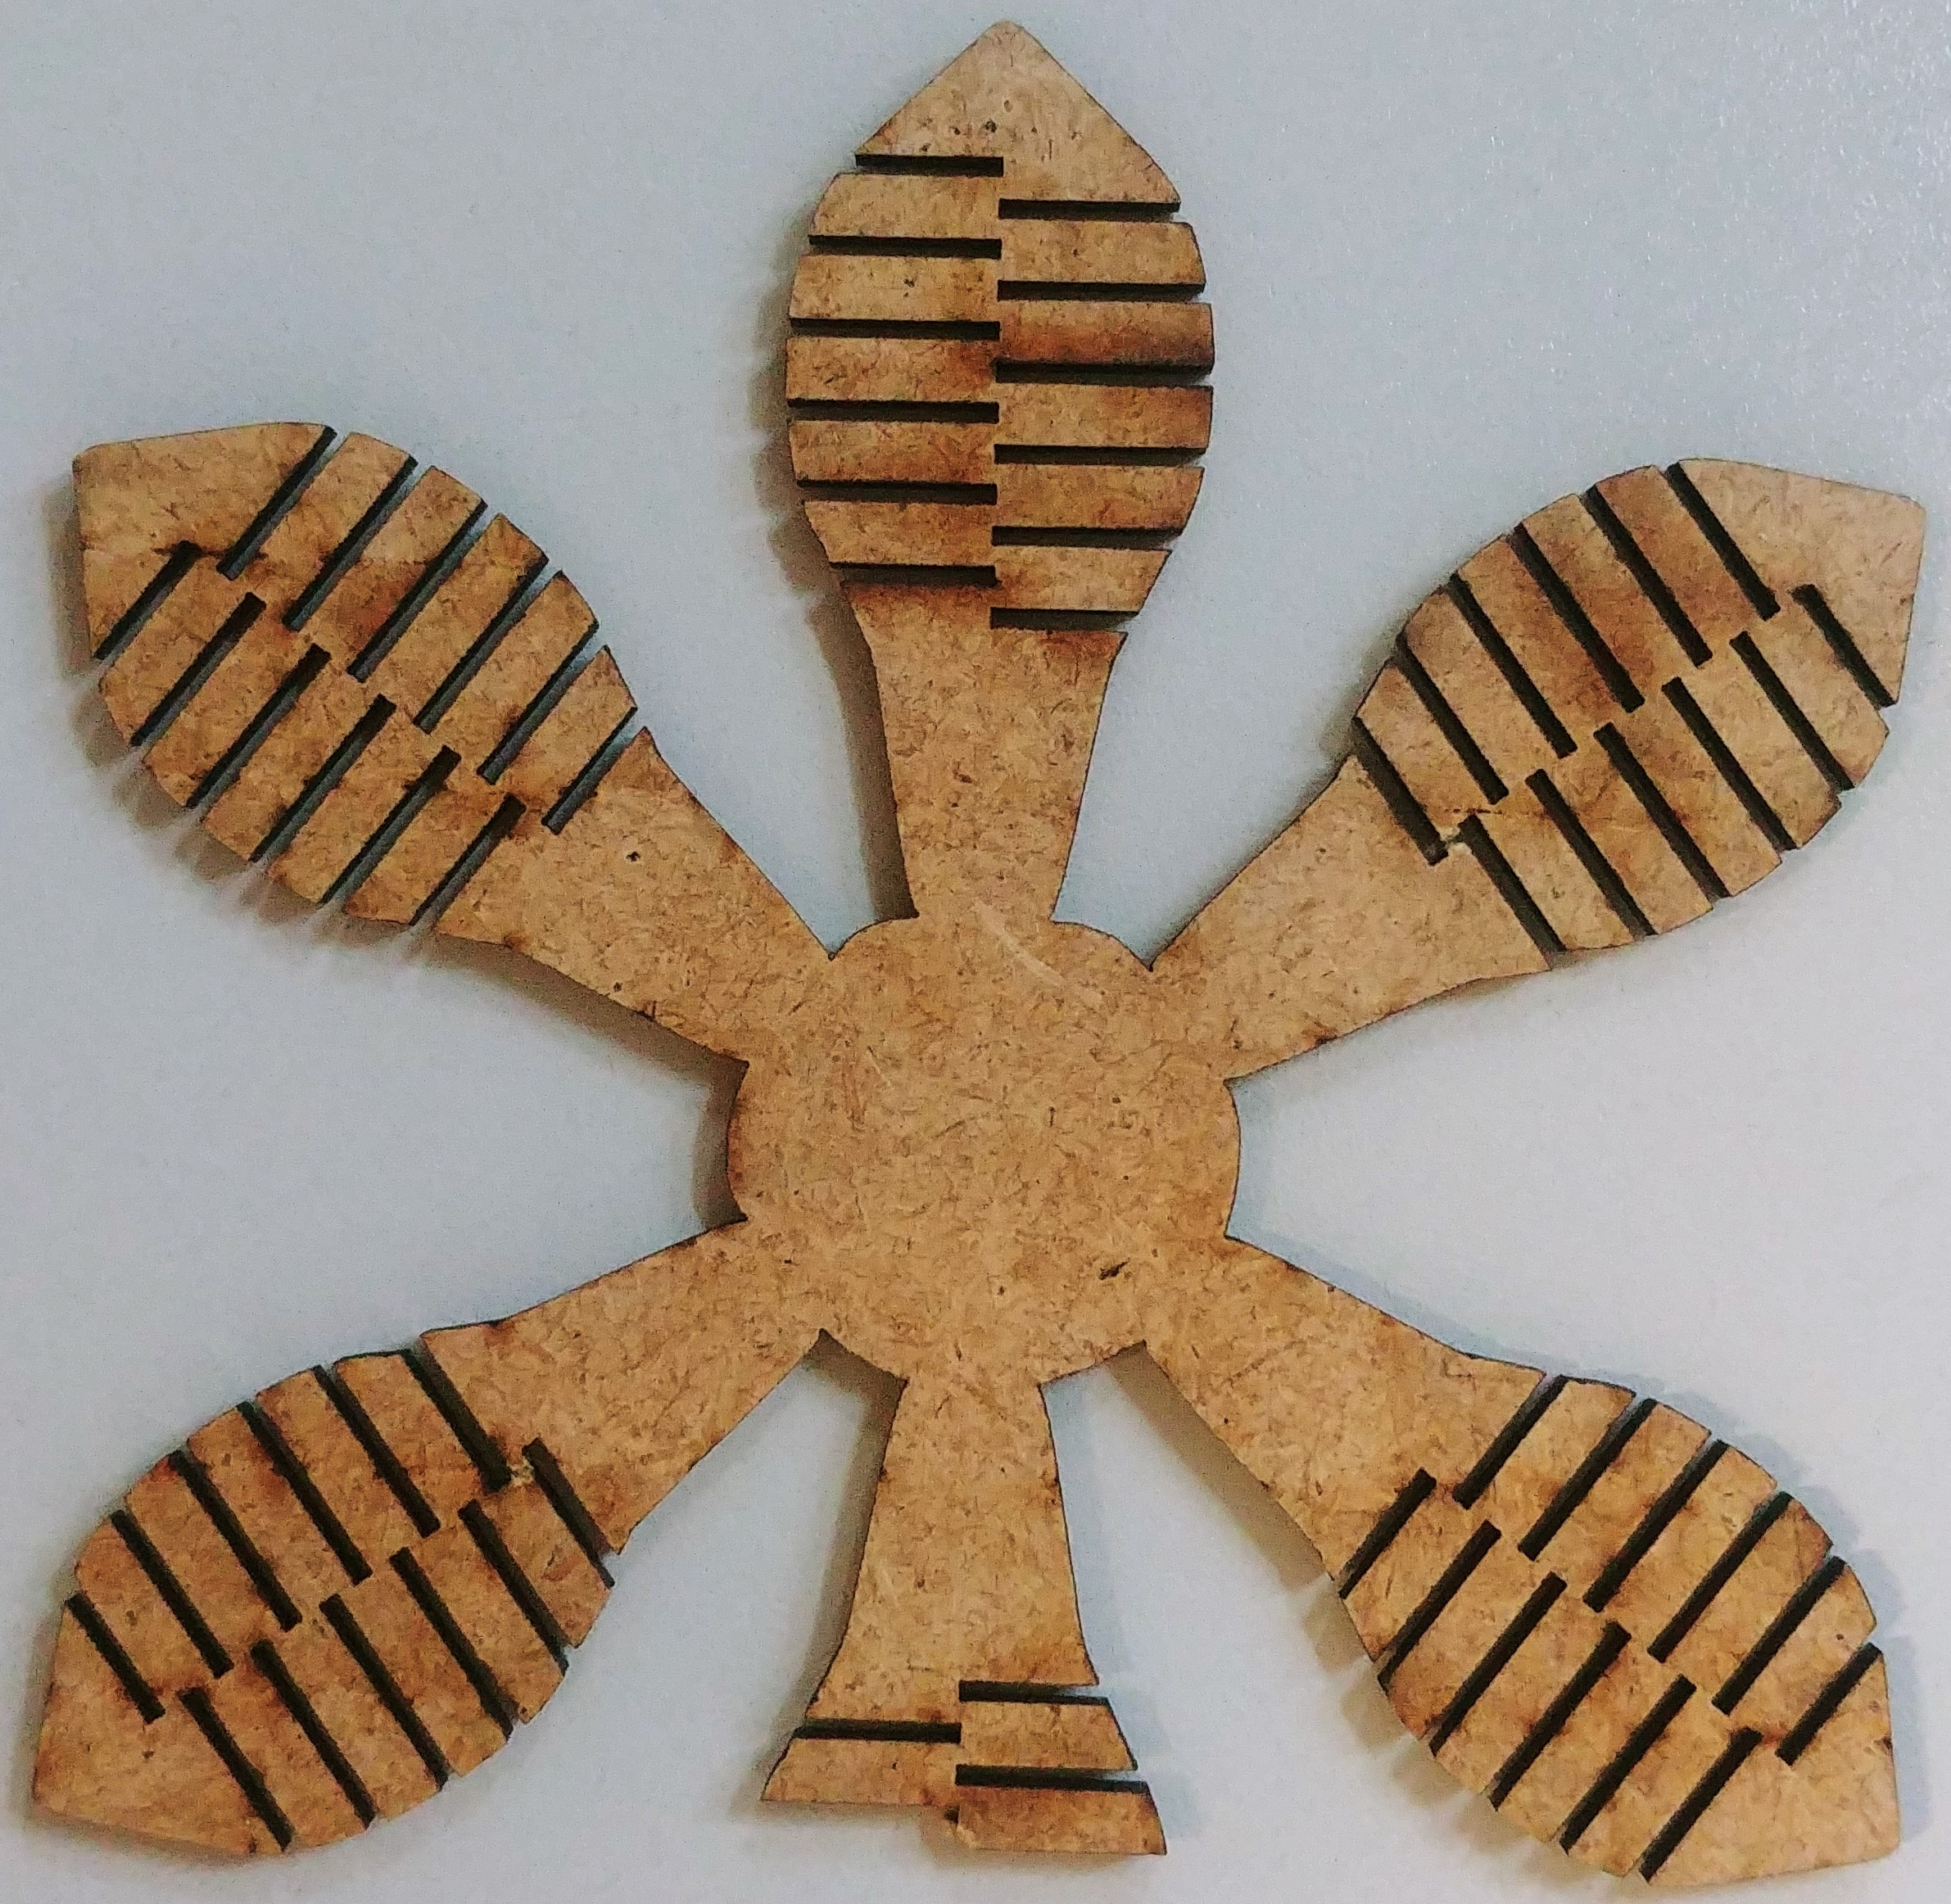
\includegraphics[width=0.6\linewidth]{images/process/03_LaserCut.jpg}
            \caption{Shows the paths that has been drilled inside of the base, so 
            users won't see any wiresing.}
            \label{fig:drillPath}
            \vspace{6mm}
        \end{subfigure}
        \caption{Shows the drilling process for the final version of the lamp.}
        \label{fig:laserCutTests}
    \end{figure}
\end{document}
